\section{Sałatka z tofu/kurczakiem*}
\bigskip
\small
\begin{minipage}{0.45\textwidth}
    \noindent \textbf{Czas:} 30 minut \\
    \textbf{Poziom trudności:} umiarkowany
\end{minipage}
\begin{minipage}{0.45\textwidth}
    \noindent \textbf{Ilość sprzątania:} średnia\\
    \textbf{Wymagany mysi sprzęt:} -
\end{minipage}
\normalsize
\vspace{0.5cm}

\begin{multicols}{2}

\subsection*{Składniki}
\begin{itemize}
    \item 1 pierś z kurczaka (lub odpowiadająca ilość tofu)
    \item mix sałat
    \item garść pomidorków koktajlowych lub 1 duży, dojrzały pomidor
    \item 1 ogórek gruntowy
    \item 0.5 czerwonej cebuli
    \item zielona cebulka wedle uznania
    \item garść kiełków brokułu (opcjonalnie)
    \item 1 duży ząbek czosnku przeciśnięty przez praskę
    \item 1 łyżka miodu
    \item przyprawy
    \item olej do smażenia
    \item odrobina oliwy i soku z cytryny
    \item sól i pieprz do smaku
\end{itemize}

\columnbreak

\begin{figure}[H]
    \centering
    \fbox{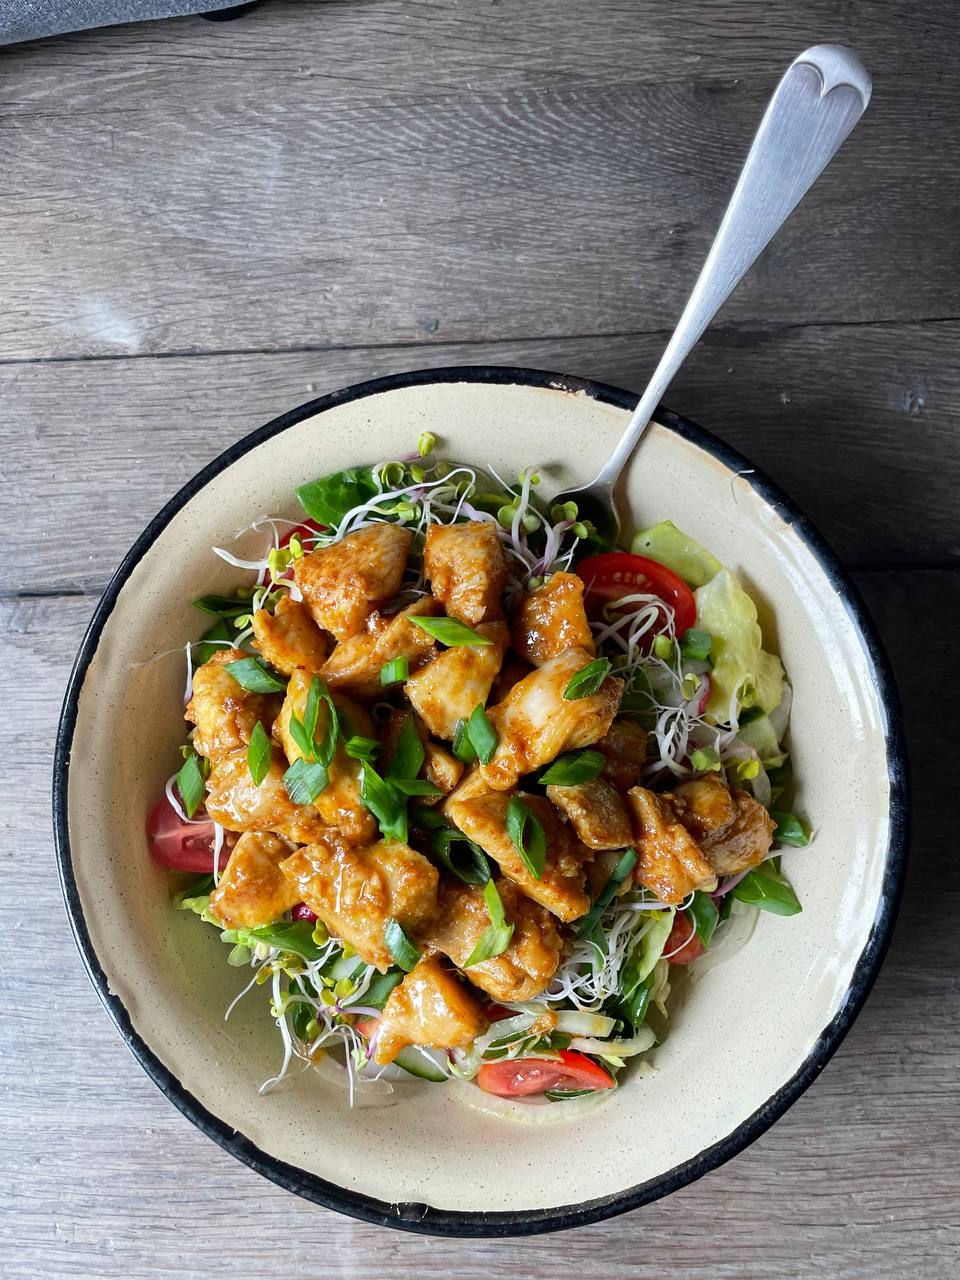
\includegraphics[width=0.4\textwidth]{images/salatka.jpg}}
\end{figure}
\end{multicols}

\vspace{0.5cm}

\subsection*{Instruktaż}
\begin{enumerate}
    \item Kurczaka/tofu pokroić w średniej wielkości kostkę, przełożyć do niewielkiej miski i doprawić po 1/2 łyżeczki solą oraz pieprzem. dołożyć czosnek i następująco po 1 płaskiej łyżeczce: oliwy, papryki słodkiej, bazylii, oregano, majeranku i przyprawy do kurczaka. wymieszać dokładnie pozostawić do marynowania na ok. 10 minut.
    \item W międzyczasie pokroić ogórka, pomidorki na połówki i cebulę w piórka. do dużej miski nałożyć garść sałaty i dosypać pokrojone wcześniej warzywa oraz kiełki. całość doprawić solą, pieprzem, oliwą i sokiem z cytryny. wszystko bardzo dokładnie wymieszać.
    \item Patelnię rozgrzać na średnim ogniu wraz z niewielką ilością oleju. kurczaka smażyć krótko, ok. 3 min na każdą stronę, aż do momentu uzyskania jednolitego koloru wewnątrz kawałków. tofu smażyć dłużej, ok. 15 minut, często mieszając, do momentu uzyskania chrupkiej warstwy zewnętrznej (można pomóc dodając 2 łyżeczki skrobii ziemniaczanej).
    \item po upływie odpowiedniego czasu zgasić palnik, doprawić kurczaka/tofu łyżką miodu, całość dokładnie wymieszać i pozostawić do ostudzenia.
    \item Na sałatę nałożyć kurczaka/tofu i posypać posiekaną zieloną cebulką.
\end{enumerate}

\vspace{0.5cm}

\small
\subsection*{Propozycja podania}
Ze świeżym pieczywem i masłem/oliwą, jako dodatek do obiadu.

\vspace{0.3cm}

\subsection*{Dodatkowe uwagi}
• do sałatki warto dodać sezonowe warzywa wedle własnego uznania, np. rzodkiewkę, paprykę, marchewkę, awokado, itp.
 • aby ostry smak surowej czerwonej cebuli nie przytłaczał pozostałych składników, warto ją sparzyć - czyli pokrojoną już w piórka wrzucić do niewielkiej miseczki i zalać wrzątkiem na kilka minut. to spowoduje, że cebula w potrawach zachowa swój pyszny smak, a jednocześnie zaniknie jej nieprzyjemna ostrość

\newpage
